\documentclass[12pt]{scrartcl}
\usepackage[sexy]{james}
\usepackage[noend]{algpseudocode}
\setlength {\marginparwidth}{2cm}
\setcounter{MaxMatrixCols}{20}
\usepackage{answers}
\usepackage{array}
\usepackage{tikz}
\newenvironment{allintypewriter}{\ttfamily}{\par}
\usepackage{listings}
\usepackage{xcolor}
\usetikzlibrary{arrows.meta}
\usepackage{color}
\usepackage{mathtools}
\newcommand{\U}{\mathcal{U}}
\newcommand{\E}{\mathbb{E}}
\usetikzlibrary{arrows}
\Newassociation{hint}{hintitem}{all-hints}
\renewcommand{\solutionextension}{out}
\renewenvironment{hintitem}[1]{\item[\bfseries #1.]}{}
\renewcommand{\O}{\mathcal{O}}
\declaretheorem[style=thmbluebox,name={Chinese Remainder Theorem}]{CRT}
\renewcommand{\theCRT}{\Alph{CRT}}
\setlength\parindent{0pt}
\usepackage{sansmath}
\usepackage{pgfplots}

\usetikzlibrary{automata}
\usetikzlibrary{positioning}  %                 ...positioning nodes
\usetikzlibrary{arrows}       %                 ...customizing arrows
\newcommand{\eqdef}{=\vcentcolon}
\newcommand{\tr}{{\rm tr\ }}
\newcommand{\im}{{\rm Im\ }}
\newcommand{\spann}{{\rm span\ }}
\newcommand{\Col}{{\rm Col\ }}
\newcommand{\Row}{{\rm Row\ }}
\newcommand{\dint}{\displaystyle\int}
\newcommand{\dt}{\ {\rm d }t}
\newcommand{\PP}{\mathbb{P}}
\newcommand{\horizontal}{\par\noindent\rule{\textwidth}{0.4pt}}
\usepackage[top=3cm,left=3cm,right=3cm,bottom=3cm]{geometry}
\newcommand{\mref}[3][red]{\hypersetup{linkcolor=#1}\cref{#2}{#3}\hypersetup{linkcolor=blue}}%<<<changed

\tikzset{node distance=4.5cm, % Minimum distance between two nodes. Change if necessary.
         every state/.style={ % Sets the properties for each state
           semithick,
           fill=cyan!40},
         initial text={},     % No label on start arrow
         double distance=4pt, % Adjust appearance of accept states
         every edge/.style={  % Sets the properties for each transition
         draw,
           ->,>=stealth',     % Makes edges directed with bold arrowheads
           auto,
           semithick}}


% Start of document.
\newcommand{\sep}{\hspace*{.5em}}

\pgfplotsset{compat=1.18}
\begin{document}
\title{MATH403: Homework 4}
\author{James Zhang\thanks{Email: \mailto{jzhang72@terpmail.umd.edu}}}
\date{\today}

\definecolor{dkgreen}{rgb}{0,0.6,0}
\definecolor{gray}{rgb}{0.5,0.5,0.5}
\definecolor{mauve}{rgb}{0.58,0,0.82}

\lstset{frame=tb,
  language=Java,
  aboveskip=3mm,
  belowskip=3mm,
  showstringspaces=false,
  columns=flexible,
  basicstyle={\small\ttfamily},
  numbers=left,
  numberstyle=\tiny\color{gray},
  keywordstyle=\color{blue},
  commentstyle=\color{dkgreen},
  stringstyle=\color{mauve},
  breaklines=true,
  breakatwhitespace=true,
  tabsize=3
}

\maketitle

\begin{center}
  
\includegraphics[width=14cm]{10.png}
\end{center}

\begin{proof}
\hfill

\begin{enumerate}
  \item Denote this permutation $\alpha$. 
  \begin{itemize}
    \item $\alpha(1) \implies$ $(13)$ sends $1$ to $3$, then $(1245)$ fixes $3$, $(13)$ sends $3$ back to $1$. 
    \item $\alpha(2) \implies (13)$ fixes $2$, $(1245)$ sends $2$ to $4$, then $(13)$ fixes $4$. 
    \item $\alpha(3) \implies (13)$ sends $3$ to $1$, $(1245)$ sends $1$ to $2$, and $(13)$ fixes $2$. 
    \item $\alpha(4) \implies (13)$ fixes $4$, $(1245)$ sends $4$ to $5$, then $(13)$ fixes $5$. 
    \item $\alpha(5) \implies (13)$ fixes $5$, $(1245)$ sends $5$ to $1$, then $(13)$ sends $1$ to $3$. 
  \end{itemize}
  This yields the disjoint cycle form $(1)(2453)$. Compared to the middle cycle $(1245) = (1245)(3)$, the product cycle 
  essentially makes $1$ the identity cycle, and replaces $1$ with $3$ in the middle cycle. 
  \item Denote this permutation $\beta$. 
  \begin{itemize}
    \item $\beta(1) \implies (24)$ fixes $1$, $(13456)$ sends $1$ to $3$, and $(24)$ fixes $3$. 
    \item $\beta(2) \implies (24)$ sends $2$ to $4$, $(13456)$ sends $4$ to $5$, and $(24)$ fixes $5$.  
    \item $\beta(3) \implies (24)$ fixes $3$, $(13456)$ sends $3$ to $4$, and $(24)$ sends $4$ to $2$. 
    \item $\beta(4) \implies (24)$ sends $4$ to $2$, $(13456)$ fixes $2$, and $(24)$ sends $2$ to $4$. 
    \item $\beta(5) \implies (24)$ fixes $5$, $(13456)$ sends $5$ to $6$, and $(24)$ fixes $6$. 
    \item $\beta(6) \implies (24)$ fixes $6$, $(13456)$ sends $6$ to $1$, and $(24)$ fixes $1$. 
  \end{itemize}
  This yields the disjoint cycle $(13256)(4)$. Compared to the middle cycle $(13456) = (13456)(2)$, the product cycle 
  essentially makes $(4)$ the identity cycle, and replaces $4$ with $2$ in the middle cycle. 
\end{enumerate}

\end{proof}
\newpage

\begin{center}
  
\includegraphics[width=14cm]{30.png}
\end{center}

\begin{proof}
  By \textbf{Theorem 5.4} in Gallian, every permutation in $S_n$ where $n > 1$ can be written as a product of two cycles. Without loss of generality, $\alpha$ omits the decomposition, 
  \[\alpha = (a_1a_k)(a_1a_{k-1}) \cdots (a_1a_2)(b_1b_t)(b_1b_{t-1}) \cdots (b_1b_2) \cdots (c_1c_2)(c_1c_{s-1})\cdots(c_1c_2)\]
  Let $k$ be the number of 2-cycles to represent the permutation $\alpha$. By \textbf{Theorem 5.5}, $k$ is either always even or always odd. 
  Similarly, let $r$ be the number of 2-cycles to represent $\beta$, which is also always even or odd. Note that if a permutation is even or odd, then the inverse of the permutation is the 
  also the same parity. Now let us take cases to show that irrespective of the parity of $\alpha$ and $\beta$, 
  the product permutaiton $a^{-1}\beta^{-1}\alpha\beta$ is always an even permutation. To do this, we will just sum the number of 
  2-cycles in the product; since \textbf{Theorem 5.5} holds, if this sum is even, then we can immediately conclude that 
  the product permutation is even. 
  \begin{enumerate}
    \item $\alpha, \beta$ are both even $\implies$ even + even + even + even $\implies$ even
    \item $\alpha$ even and $\beta$ odd $\implies$ even + odd + even + odd $\implies$ even
    \item $\alpha$ odd and $\beta$ even $\implies$ odd + even + odd + even $\implies$ even
    \item $\alpha, \beta$ both odd $\implies$ odd + odd + odd + odd $\implies$ even
  \end{enumerate}
  Therefore, the product cycle $\alpha^{-1}\beta^{-1}\alpha\beta$ is an even permutation, as desired.
\end{proof}
\newpage

\begin{center}
  
\includegraphics[width=14cm]{40.png}
\end{center}

\begin{proof}

  Given that $\beta^1 = (123)(145)$, note that $1\to 4, 2 \to 3, 3 \to 1, 4 \to 5, 5 \to 2, 6 \to 6$ and so the disjoint cycle form 
  is
  \[\beta^1 = (123)(145) \implies (14523)\]
  This cycle is of order $5$, so therefore, $\beta^1 = \beta^6$. Note that $99 \equiv 4 \text{ mod } 5$. Therefore, 
  \[\beta^{99} = \beta^4 = (14523)(14523)(14523)(14523)\]
  and since $1 \to 3, 2 \to 5, 3 \to 2, 4 \to 1, 5 \to 4$, and this implies that 
  \[\beta^{99} = (13254)\]
\end{proof}
\newpage

\begin{center}
  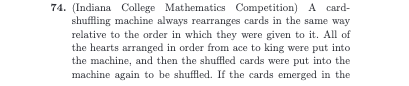
\includegraphics[width=14cm]{74.png}
  
\includegraphics[width=11cm]{74p2.png}
\end{center}

\begin{proof}
  Let us denote the rank of the card numerically such that $A = 1, 2=2 \cdots, K = 13$. 
  We seek a permutation 
\[\alpha = \begin{bmatrix}
    1 & 2 & 3 & 4 & 5 & 6 & 7 & 8 & 9 & 10 & 11 & 12 & 13\\
    \alpha_1 & \alpha_2 & \alpha_3 & \alpha_4 & \alpha_5 & \alpha_6 & \alpha_7 & \alpha_8 & \alpha_9 & \alpha_{10} & \alpha_{11} & \alpha_{12} & \alpha_{13}
  \end{bmatrix}\]
  such that 
\[\alpha^2 = \begin{bmatrix}
    1 & 2 & 3 & 4 & 5 & 6 & 7 & 8 & 9 & 10 & 11 & 12 & 13\\
    10 & 9 & 12 & 8 & 13 & 3 & 4 & 1 & 5 & 11 & 6 & 2 & 7
  \end{bmatrix}\]
  and from here, the sequence $\alpha_1, \ldots, \alpha_{13}$ will be the order of the cards after the first shuffle. Note, however, that since the card-shuffling 
  machine always rearranges card in the same relative order, $\alpha^{13}$ will be the identity. Thus, to find the order after the first shuffle, we need only find the 
  order after the $14th$ shuffle, and this will be the same order. To do this, we must apply $\alpha^2$ six more times. 
  To help with this, I wrote a simple Python script to find the order after $\alpha^{14} = \alpha^{1}$. 

  \begin{lstlisting}[language=Python]
alpha_squared = {1: 10, 2: 9, 3: 12, 4: 8, 5: 13, 6: 3, 7: 4, 8: 1, 9: 5, 10: 11, 11: 6, 12: 2, 13: 7}
curr = {i: i for i in range(1, 14)}
for i in range(7):
  curr = {j: curr[alpha_squared[j]] for j in range(1, 14)}
print(curr)
  \end{lstlisting}
The result of \verb|curr| is \verb|{1: 9, 2: 1, 3: 4, 4: 12, 5: 11, 6: 7, 7: 3, 8: 2|

\verb|, 9: 10, 10: 5, 11: 13, 12: 8, 13: 6}|. Converting this back to our cards ranks, we obtain that the original order of the 
cards is 
\[9, A, 4, Q, J, 7, 3, 2, 10, 5, K, 8, 6\]
\end{proof}
\newpage

\begin{center}
  
\includegraphics[width=14cm]{30_6.png}
\end{center}

\begin{proof}
  Let $\alpha: \textbf{R}^* \to \textbf{R}^*$ be a mapping such that we have an automorphism of $\textbf{R}^*$ --- 
  then it follows that $\alpha$ is 1-1, onto, and operation preserving. Furthermore, by \textbf{Property 1 of Theorem 6.1}, 
  $\alpha$ carries the identity of $\textbf{R}^*$ to the identity of $\textbf{R}^*$. Therefore, we have 
  \[\alpha(1) = 1\]
  Since $-1 \in \textbf{R}^*$, we can apply the automorphism 
  \[1 = \alpha(1) = \alpha(-1 * -1) = \alpha(-1) \alpha(-1)\]
  which implies that $\alpha(-1) = -1, 1$. However, $\alpha$ is 1-1, and therefore, 
  \[\alpha(-1) = \alpha(1) \implies -1 = 1\]
  which is a contradiction. Therefore, $\alpha(-1) = -1$ must be true to satisfy the definition of automorphism, as desired. 
\end{proof}
\newpage

\begin{center}
  
\includegraphics[width=14cm]{48.png}
\end{center}

\begin{proof}
  Assume on the contrary that there exists a function $\phi: \textbf{R} \to \textbf{R}^*$ such that 
  $\textbf{R}$ under addition is isomorphic to $\textbf{R}^*$ under multiplication. Then, it follows that 
  $\phi$ is both 1-1, onto, and operation-preserving. If $\phi$ were such a mapping, there would 
  exist a real number $x \in \textbf{R}$ such that $\phi(x) = -1$ as $-1 \in \textbf{R}^*$. However, observe that 
  \[-1 = \phi(x) = \phi\left(\frac{1}{2}x + \frac{1}{2}x\right) = \phi\left(\frac{1}{2}x\right)\phi\left(\frac{1}{2}x\right) = \left(\phi\left(\frac{1}{2}x\right) \right)^2\]
  However, no real number squared is $-1$ and so we've arrived at a contradiction. Therefore, 
  $\textbf{R}$ under addition is not isomorphic to $\textbf{R}^*$ under multiplcation as desired.  
\end{proof}
\newpage

\begin{center}
  
\includegraphics[width=14cm]{68.png}
\end{center}

\begin{proof}
  Let $\phi: Q \to Q$ be a mapping such that it is an automorphism of the rational numbers $Q$ under addition. 
  Therefore, $\phi$ is 1-1, onto, and operation-preserving. Furthermore, by \textbf{Property 1 of Theorem 6.1}, the identity carries through the mapping, and so
  \[\phi(0) = 0\]
  For any rational number $x \in Q$, we can write it as $x = \frac{p}{q}, p, q \in \ZZ$ and $q \neq 0$. 
  By applying the automorphism and the property of preserving operations, 
  \[\phi(x) = \phi\left(\frac{p}{q}\right) = \phi\left(p * \frac{1}{q}\right)\]
  \textbf{Property 2 of Theorem 6.1} states that for every integer $n$ group element $a \in G$, then $\phi(a^n) = [\phi(a)]^n$. Denote this result as \textbf{*}. Furthermore, in the additive form, 
  $\phi(na) = n\phi(a)$. Denote this result as \textbf{**}.
  Therefore, in our context, since $p \in \ZZ$ and $\frac{1}{q} \in Q$, we can apply \textbf{**}
  \[\phi\left(p * \frac{1}{q}\right) = p\phi\left(\frac{1}{q}\right)\] 
  Now applying \textbf{*} because $q$ is in the group of rationals and $-1$ is an integer 
  \[p\phi\left(\frac{1}{q}\right) = p\phi(q^{-1}) = p[\phi(q)]^{-1} = p * \frac{1}{\phi(q)}\]
  Applying \textbf{**} once more, 
  \[p * \frac{1}{\phi(q * 1)} = p * \frac{1}{q \phi(1)} = \frac{p}{q} [\phi(1)]^{-1}\]
  By \textbf{*} for the last time, since $-1$ is an integer and $1 \in Q$, 
  \[= \frac{p}{q}\phi(1^{-1}) = \frac{p}{q}\phi\left(\frac{1}{1}\right) = \frac{p}{q}\phi(1) = x\phi(1)\]
  and thus we have shown that for any automorphism $\phi$ of the rational numbers $Q$ under addition, and 
  for any $x \in Q$
  \[\phi(x) = x\phi(1)\]
  as desired. 
\end{proof}

\end{document}

